\documentclass[ignorenonframetext,]{beamer}
\setbeamertemplate{caption}[numbered]
\setbeamertemplate{caption label separator}{: }
\setbeamercolor{caption name}{fg=normal text.fg}
\usepackage{lmodern}
\usepackage{amssymb,amsmath}
\usepackage{ifxetex,ifluatex}
\usepackage{fixltx2e} % provides \textsubscript
\ifnum 0\ifxetex 1\fi\ifluatex 1\fi=0 % if pdftex
  \usepackage[T1]{fontenc}
  \usepackage[utf8]{inputenc}
\else % if luatex or xelatex
  \ifxetex
    \usepackage{mathspec}
  \else
    \usepackage{fontspec}
  \fi
  \defaultfontfeatures{Ligatures=TeX,Scale=MatchLowercase}
  \newcommand{\euro}{€}
\fi
% use upquote if available, for straight quotes in verbatim environments
\IfFileExists{upquote.sty}{\usepackage{upquote}}{}
% use microtype if available
\IfFileExists{microtype.sty}{%
\usepackage{microtype}
\UseMicrotypeSet[protrusion]{basicmath} % disable protrusion for tt fonts
}{}
\newif\ifbibliography
\usepackage{graphicx,grffile}
\makeatletter
\def\maxwidth{\ifdim\Gin@nat@width>\linewidth\linewidth\else\Gin@nat@width\fi}
\def\maxheight{\ifdim\Gin@nat@height>\textheight0.8\textheight\else\Gin@nat@height\fi}
\makeatother
% Scale images if necessary, so that they will not overflow the page
% margins by default, and it is still possible to overwrite the defaults
% using explicit options in \includegraphics[width, height, ...]{}
\setkeys{Gin}{width=\maxwidth,height=\maxheight,keepaspectratio}

% Prevent slide breaks in the middle of a paragraph:
\widowpenalties 1 10000
\raggedbottom

% Comment these out if you don't want a slide with just the
% part/section/subsection/subsubsection title:
\AtBeginPart{
  \let\insertpartnumber\relax
  \let\partname\relax
  \frame{\partpage}
}
\AtBeginSection{
  \ifbibliography
  \else
    \let\insertsectionnumber\relax
    \let\sectionname\relax
    \frame{\sectionpage}
  \fi
}
\AtBeginSubsection{
  \let\insertsubsectionnumber\relax
  \let\subsectionname\relax
  \frame{\subsectionpage}
}

\setlength{\emergencystretch}{3em}  % prevent overfull lines
\providecommand{\tightlist}{%
  \setlength{\itemsep}{0pt}\setlength{\parskip}{0pt}}
\setcounter{secnumdepth}{0}

\title{Regression Fit}
\author{Jeffrey Arnold}
\date{May 10, 2016}
\usepackage{amsmath}
\usepackage{amsfonts}
\DeclareMathOperator{\E}{E}
\DeclareMathOperator{\mean}{mean}
\DeclareMathOperator{\Var}{Var}
\DeclareMathOperator{\Cov}{Cov}
\DeclareMathOperator{\Cor}{Cor}
\DeclareMathOperator{\Bias}{Bias}
\DeclareMathOperator{\MSE}{MSE}
\DeclareMathOperator{\sd}{sd}
\DeclareMathOperator{\se}{se}
\DeclareMathOperator{\rank}{rank}
\DeclareMathOperator*{\argmin}{arg\,min}
\DeclareMathOperator*{\argmax}{arg\,max}

\newcommand{\mat}[1]{\boldsymbol{#1}}
\renewcommand{\vec}[1]{\boldsymbol{#1}}
%\renewcommand{\T}{'}

\newcommand{\distr}[1]{\mathcal{#1}}
\newcommand{\dnorm}{\distr{N}}
\newcommand{\dmvnorm}[1]{\distr{N}_{#1}}

\begin{document}
\frame{\titlepage}

\begin{frame}{Ways to understand model fit and advice on what to do}

\begin{enumerate}[<+->]
\def\labelenumi{\arabic{enumi}.}
\tightlist
\item
  Standard error of the regression
\item
  R-squared
\item
  Adjusted R-squared
\item
  F-test
\item
  Advice
\item
  More \ldots{}
\end{enumerate}

\end{frame}

\begin{frame}{R\^{}2}

\end{frame}

\begin{frame}{Several definitions of \(R^2\)}

\begin{itemize}[<+->]
\item
  Ratio of variance of fitted values to sample \(y\) \[
  R^2 = \frac{\Var(\hat{\vec{y}})}{\Var{\vec{y}}}
  \]
\item
  Ratio of variance ``explained'' by the regression \[
  R^2 = 1 - SSE / SST = 1 - \frac{\sum (y_i - \hat{y}_i)^2}{\sum (y_i - \bar{\vec{y}})^2}
  \]
\item
  For bivariate regression, correlation of \(Y\) and \(X\) squared, \[
  R^2 = \Cor(\vec{x}, \vec{y})^2 = \hat{\beta}_1 \frac{\sd{\vec{y}}}{\sd{\vec{x}}}
  \]
\item
  \(R^2 \in [0, 1]\) where \(1\) is all points are on a line/plane
\end{itemize}

\end{frame}

\begin{frame}{R-squared is dependent on scale of \(X\)}

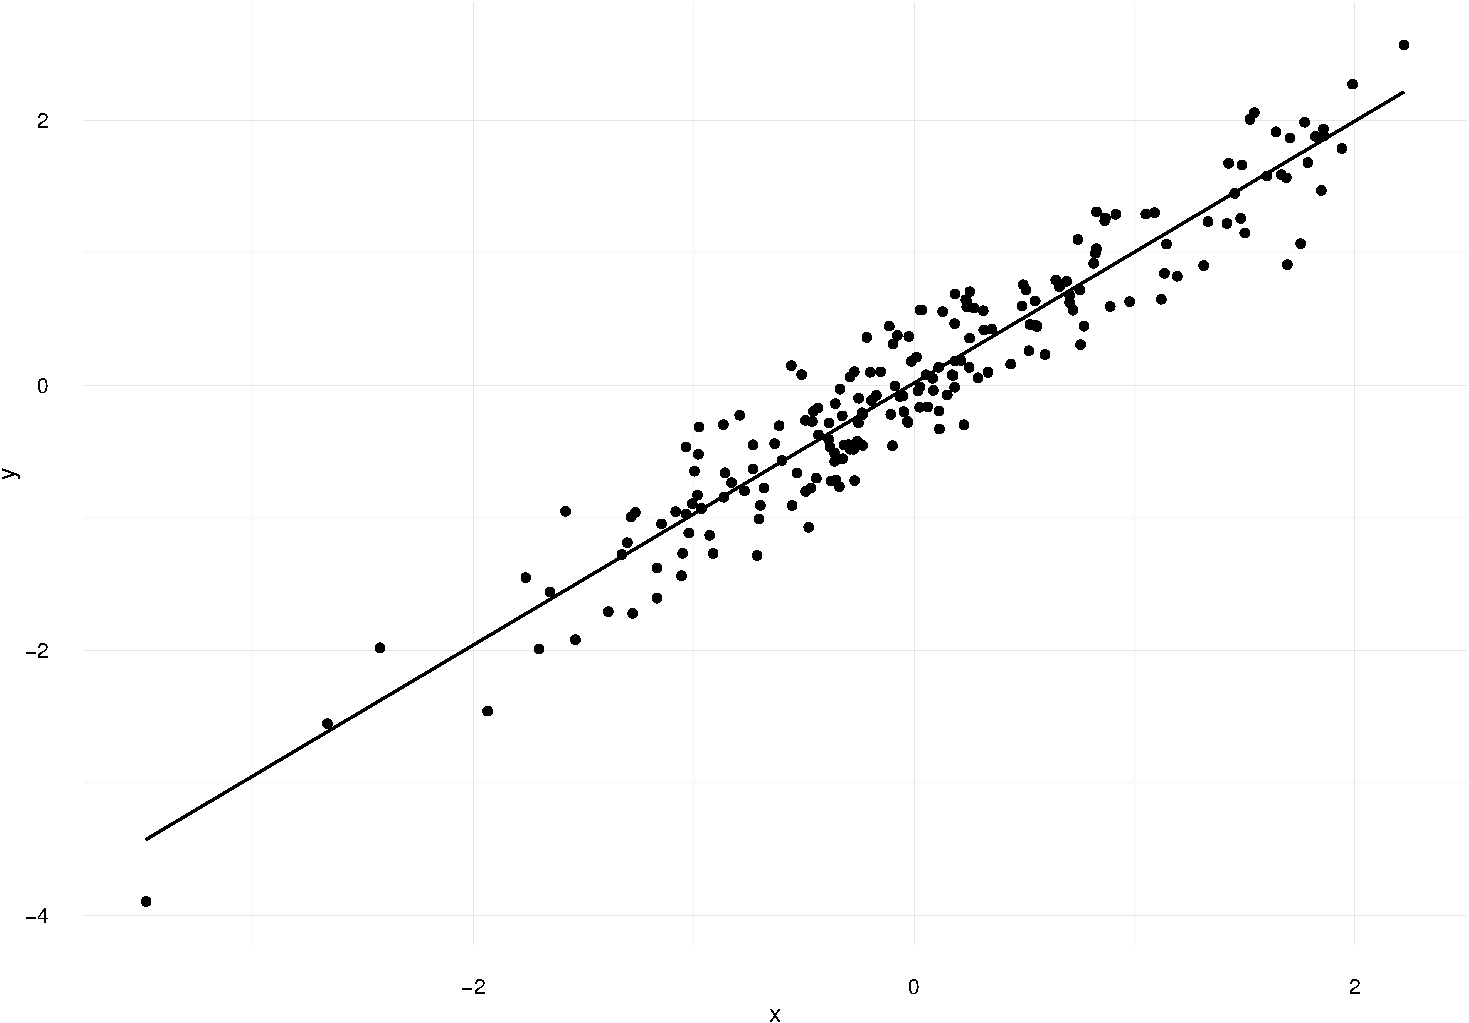
\includegraphics{r2_regression_fit_files/figure-beamer/unnamed-chunk-2-1.pdf}

\(\hat{\sigma}^2 = 0.3\), \(R^2 = 0.91\)

\end{frame}

\begin{frame}{R-squared is dependent on scale of \(X\)}

Same data, regression on subset

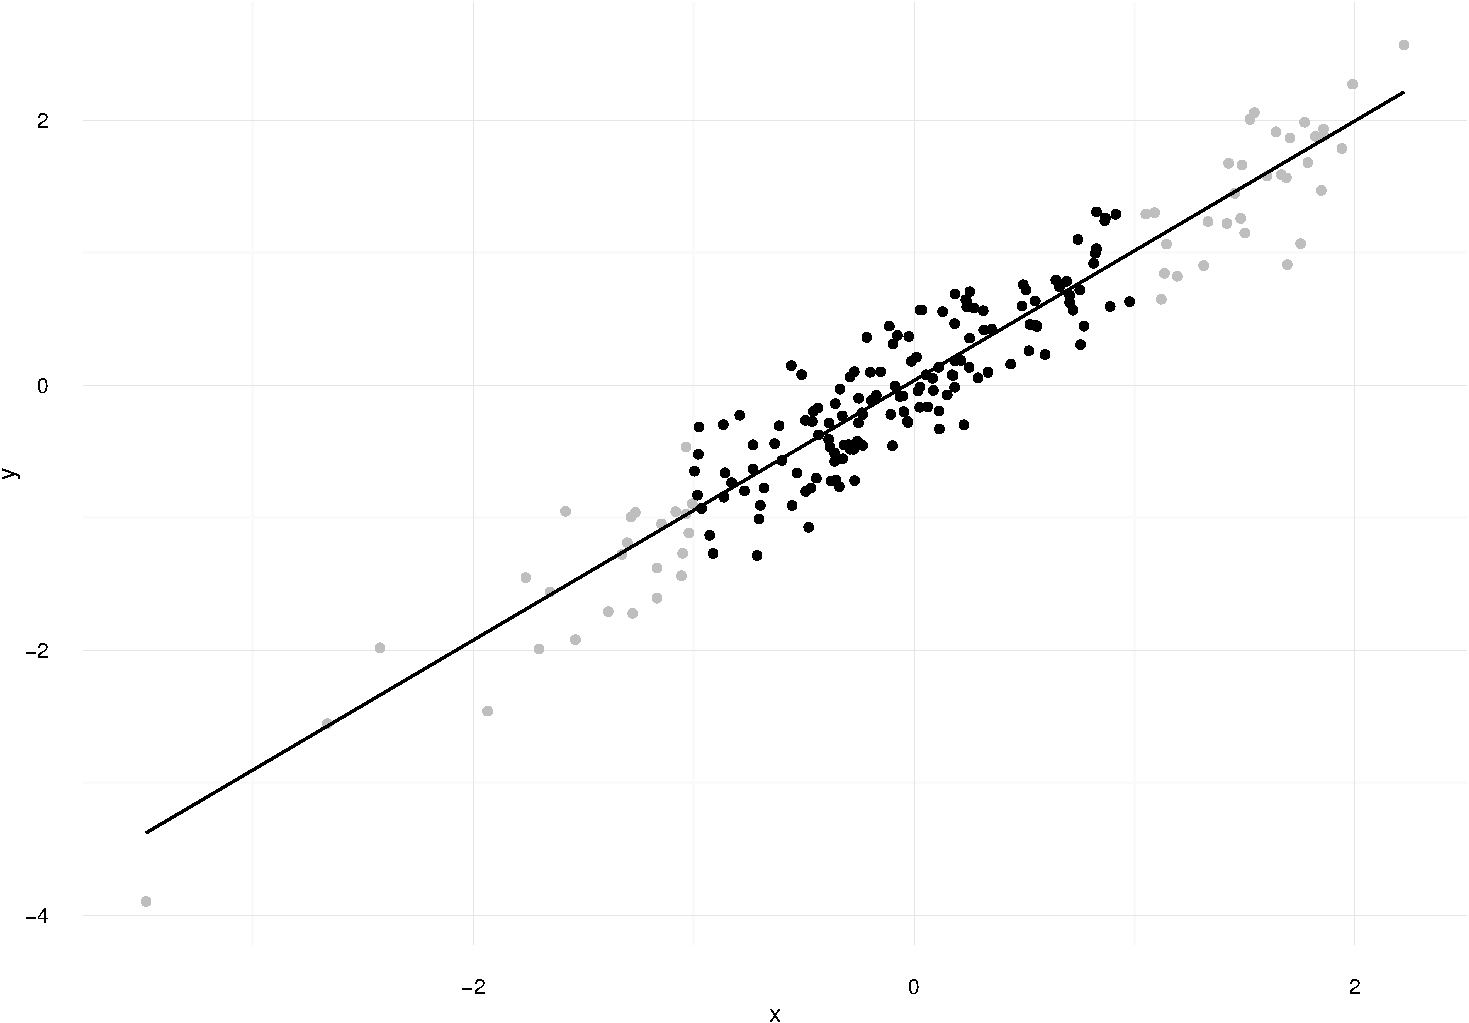
\includegraphics{r2_regression_fit_files/figure-beamer/unnamed-chunk-3-1.pdf}

\(\hat{\sigma}^2 = 0.29\), \(R^2 = 0.75\)

\end{frame}

\begin{frame}{In-sample fit always increases as variables are added}

\(y = x + \epsilon\), \(\epsilon_i \sim N(0, 2)\)

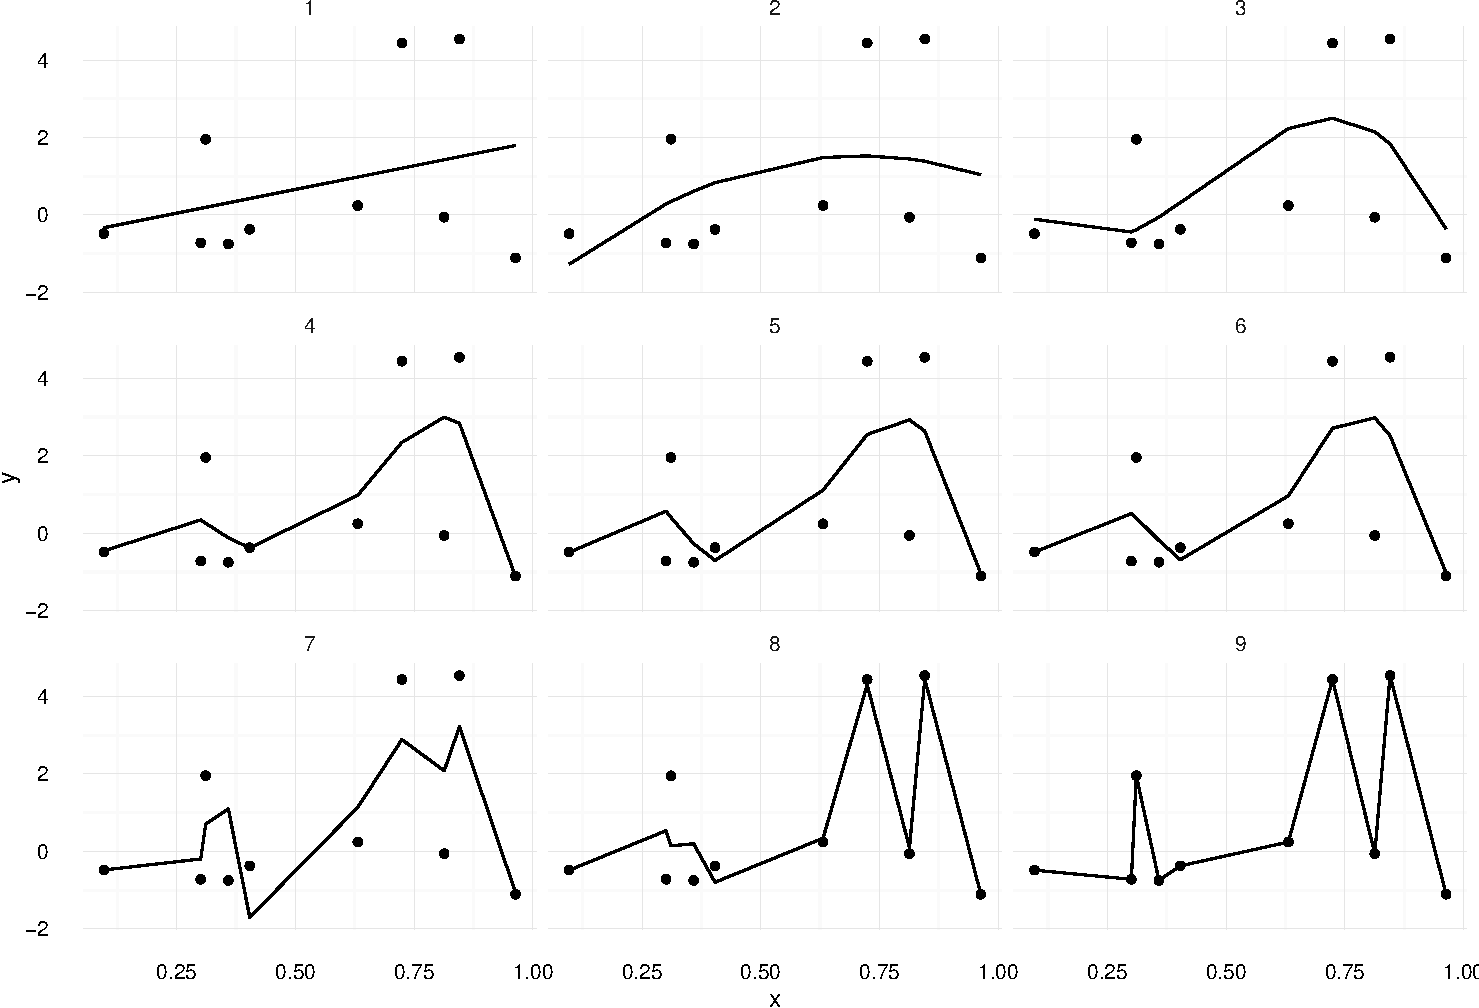
\includegraphics{r2_regression_fit_files/figure-beamer/unnamed-chunk-5-1.pdf}

\end{frame}

\begin{frame}{R-squared always increases as variables are added}

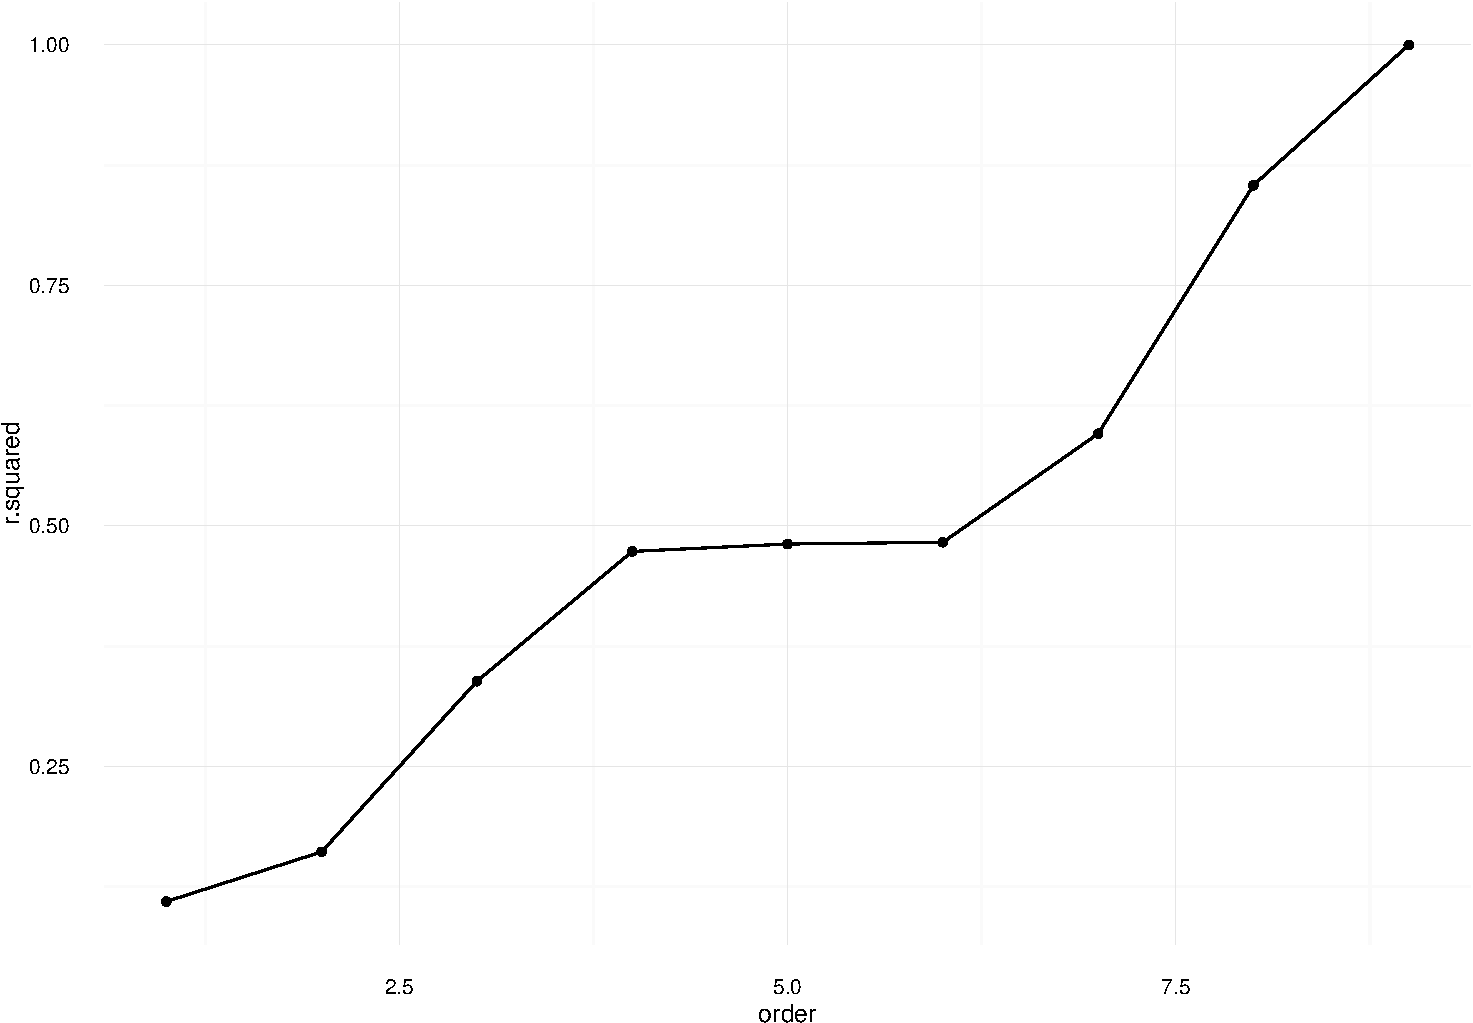
\includegraphics{r2_regression_fit_files/figure-beamer/unnamed-chunk-6-1.pdf}

\end{frame}

\begin{frame}{Other problems with R\^{}2}

\begin{enumerate}[<+->]
\def\labelenumi{\arabic{enumi}.}
\tightlist
\item
  Does not measure goodness of fit

  \begin{enumerate}[<+->]
  \def\labelenumii{\arabic{enumii}.}
  \tightlist
  \item
    To get \(R^2\) large, make \(X\) spread out
  \item
    To get \(R^2\) small, make \(X\) not spread out
  \end{enumerate}
\item
  Does not measure prediction
\item
  Cannot compare different datasets (including transformed \(Y\))
\item
  Not variance ``explained'' in causal sense
\end{enumerate}

\end{frame}

\begin{frame}{Standard error of the regression (\(\hat{sigma}\))}

\[
\hat{\sigma} = \sqrt{ \frac{1}{N - K - 1} \sum \varepsilon_i^2 }
\]

\begin{itemize}[<+->]
\tightlist
\item
  ``Average'' error
\item
  RMSE is similar, with denominator \(N\) instead of \(N - K - 1\).
\item
  On the same scale as \(\vec{y}\)
\item
  Often suggested as alternative to \(R^2\)
\end{itemize}

\end{frame}

\begin{frame}{Adjusted \(R^2\)}

Adjust \(R^2\) for sample size and variables, \[
R^2 = 1 - \frac{SSE / (N - K - 1)}{SST / (N - 1)}
\]

\begin{itemize}[<+->]
\tightlist
\item
  Slightly penalizes \(R^2\) for more variables
\item
  Adjustment only relevant for cases where \(N \approx K\)
\item
  No theory as to what it is good for
\item
  Doesn't fix any important problem with \(R^2\). Pointless for
  comparing models
\end{itemize}

\end{frame}

\begin{frame}{Problems with \(\hat{\sigma}\)}

\begin{enumerate}[<+->]
\def\labelenumi{\arabic{enumi}.}
\tightlist
\item
  Less affected by changes in scale of \(X\)
\item
  But almost all problems with R\^{}2 related to in-sample performance
\item
  To interpret \(\hat{\sigma}\) need to compare to scale (variance) of
  \(\vec{y}\), but then almost the same as \(R^2\).
\end{enumerate}

\end{frame}

\begin{frame}{\(F\)-test}

\begin{itemize}[<+->]
\tightlist
\item
  \(R^2\) and \(\hat{sigma}\) are statistics, but generally not used in
  tests
\item
  \(F\)-test with \(H_O: \beta_1 = \dots = \beta_K = 0\)
\item
  \(F\)-statistic is a function of the SSE of models
\item
  Inherits most of the same problems as \(R^2\)
\item
  Assumes that linear model is correct, not whether it is a good model
\end{itemize}

\end{frame}

\begin{frame}{What to do about it?}

\begin{enumerate}[<+->]
\def\labelenumi{\arabic{enumi}.}
\tightlist
\item
  Focus on what's important:

  \begin{enumerate}[<+->]
  \def\labelenumii{\arabic{enumii}.}
  \item
    If prediction: out of sample performance
  \item
    If causation:

    \begin{itemize}[<+->]
    \tightlist
    \item
      identification of \(\beta\) (omitted variable bias or design)
    \item
      assumptions of model (other diagnostics)
    \end{itemize}
  \end{enumerate}
\item
  Focus on results/average of many models - not the ``best'' model
\end{enumerate}

\end{frame}

\begin{frame}{Next time}

Comparing predictive performance of models using cross-validation

\end{frame}

\begin{frame}{References}

\begin{itemize}[<+->]
\tightlist
\item
  Gary King ``\href{http://gking.harvard.edu/files/mist.pdf}{How Not to
  Lie With Statistics: Avoiding Common Mistakes in Quantitative
  Political Science}.''
\item
  Cosmo Shalizi,
  \href{http://www.stat.cmu.edu/~cshalizi/mreg/15/lectures/10/lecture-10.pdf}{F-Tests,
  R2 ad, and Other Distractions}.
\item
  \href{http://andrewgelman.com/2007/08/29/rsquared_useful/}{R-squared:
  useful or evil?}
\end{itemize}

\end{frame}

\end{document}
